\documentclass[12pt,a4paper]{report}

% Page layout: UniBo page says 2 cm margins.
\usepackage[a4paper,margin=2cm]{geometry}

% Times-like font.
\usepackage{newtxtext}
\usepackage{newtxmath}

% Line spacing: UniBo allows 1 or 1.5.
\usepackage{setspace}
\onehalfspacing
\setlength{\parindent}{0pt}
\setlength{\parskip}{0.8em}

% Core packages.
\usepackage[T1]{fontenc}
\usepackage[utf8]{inputenc}
\usepackage[english]{babel}
\usepackage{graphicx}
\usepackage{booktabs}
\usepackage{float}
\usepackage{amsmath}
\usepackage{hyperref}
\renewcommand{\bibname}{References}

% Cleaner hyperlinks.
\hypersetup{
    colorlinks=true,
    linkcolor=black,
    citecolor=black,
    urlcolor=blue
}

% Thesis metadata.
\newcommand{\ThesisTitle}{Strategy Optimization via Synthetic Market Generation}
\newcommand{\AuthorName}{Jacopo Michelacci}
\newcommand{\SupervisorName}{Prof. Giovanni Cardillo}
\newcommand{\DegreeProgramme}{Bachelor's Degree in Management and Economics}
\newcommand{\AcademicYear}{2025/2026}

\begin{document}

\hypersetup{pageanchor=false}
\begin{titlepage}
    \begin{center}
        {\Large Alma Mater Studiorum -- Universit\`a di Bologna}

        \vspace{0.8cm}

        {\large \DegreeProgramme}

        \vspace{2.5cm}

        {\Huge\bfseries \ThesisTitle}

        \vfill

        \begin{minipage}{0.45\textwidth}
            \raggedright
            Supervisor:\\
            \SupervisorName
        \end{minipage}
        \hfill
        \begin{minipage}{0.45\textwidth}
            \raggedleft
            Candidate:\\
            \AuthorName
        \end{minipage}

        \vspace{2cm}

        Academic Year \AcademicYear
    \end{center}
\end{titlepage}
\hypersetup{pageanchor=true}

\pagenumbering{roman}

\chapter*{Abstract}
\addcontentsline{toc}{chapter}{Abstract}
This thesis studies the problem of robust strategy optimization in systematic trading. The central
question is how trading strategies can be optimized on past market data while limiting the risk of
overfitting, but more specifically, which optimization procedure produces more reliable
out-of-sample performance.

To address this question, the project develops an efficient research framework composed of a C++
backtesting and optimization engine linked to Python reporting and analysis tools. The C++ component
is responsible for data processing, strategy simulation, trade reconstruction, and grid-based
parameter optimization. The Python component is used for plotting, report generation, and
performance analysis. This separation allows the computationally intensive parts of the workflow to
remain efficient and independent, while keeping the analytical layer flexible.

The empirical analysis uses the same discretionary optimization procedure under two different
data-generation settings. The benchmark approach optimizes the strategy on the historical in-sample
period, defined as the first 70\% of the original series. The alternative approach optimizes the
strategy on synthetic markets generated from the same in-sample window: multiple synthetic paths are
produced, the strategy is evaluated across them, and parameter selection is based on average
performance rather than on a single historical path. In both cases, parameter selection is performed
using discretion, following basic robustness principles rather than blindly selecting the single
best result. The selected parameters are then frozen and tested on the same out-of-sample period,
corresponding to the final 30\% of the original historical series. The comparison focuses on the gap
between optimization performance and out-of-sample performance: a smaller deterioration is
interpreted as evidence of lower overfitting.

The results do not show a clear reduction in overfitting from the synthetic optimization method. The
synthetic paths are useful as alternative market scenarios, but in these experiments they do not lead
to parameters that generalize better than the standard IS/OOS benchmark.


\tableofcontents
\clearpage

\pagenumbering{arabic}

\chapter{Introduction}
\section{Motivation}

Systematic trading strategies are rules that transform market data into trading decisions. Their
appeal is straightforward: if a set of rules can identify repeatable market patterns, or possible
market inefficiencies, it may be used to improve returns, control risk, and reduce dependence on
discretionary judgement. Most strategies contain parameters, such as lookback windows, thresholds,
or position-sizing rules. The process of choosing these parameters is known as strategy
optimization, and it is a central part of algorithmic trading research. When performed carefully,
optimization can help identify more effective configurations; when performed naively, it can lead to
misleading results and poor live performance.

The difficulty is that better historical performance does not automatically imply better future
performance. In financial markets, the familiar warning that past returns are not indicative of
future returns is not a legal formality only; it reflects a real statistical problem. A strategy can
perform well in a backtest because it captures a genuine and persistent market effect, but it can
also perform well simply because its parameters were fitted too closely to the specific historical
sample being tested. This second case is the problem of overfitting, which is perhaps the most
common and insidious challenge that one can tackle in strategy optimization.

\section{The overfitting problem}

A naive approach to strategy development would be to optimize a strategy on the full available
historical dataset and then deploy the best-performing configuration. This is problematic because
the same data is used both to choose the parameters and to judge the quality of the strategy. If
many parameter combinations are tested, some of them are likely to look good by chance, even if the
underlying rule has little predictive value. The more parameter combinations and strategy variations
are tested, the greater the probability of finding a configuration that performed well on the
historical sample by chance rather than because of a robust underlying effect. Such a configuration
may produce an impressive backtest, but fail when applied to new market data.

Overfitting can therefore be understood as a loss of generalization. The strategy becomes too
adapted to the noise, anomalies, and specific sequence of events observed in the historical sample.
As a consequence, the more a strategy is overfitted, the less likely it is that its backtested
performance will be repeated in the future.

A common response to this issue is to split the historical data into two parts. The first part,
usually called the in-sample period (IS from now on), is used to develop and optimize the strategy.
The second part, called the out-of-sample period (OOS from now on), is kept separate and used only
after the parameters have been selected. In this thesis, the benchmark approach uses a 70\%
in-sample and 30\% out-of-sample split, where the out-of-sample period corresponds to the most
recent part of the original historical series. This reflects the practical objective of testing
whether a strategy optimized on the past would have remained effective on later unseen data.

\section{Research question}

The central question of this thesis is whether a synthetic-market-based optimization procedure can
improve robustness compared with the standard historical in-sample optimization approach. Both
methods use the same general optimization logic, but they differ in the data on which the
optimization is performed.

In the benchmark case, the strategy is optimized directly on the historical in-sample period. In the
synthetic case, the in-sample period is first used to generate multiple synthetic market paths. The
strategy is then optimized across these generated paths, and parameter selection is based on average
results rather than on one realized historical path. The selected parameters from both approaches
are finally tested on the same real out-of-sample period. This makes the comparison focused: the
objective is not to prove that a strategy is profitable, but to evaluate which optimization
procedure loses less performance when moving from optimization to OOS testing.

\section{Approach and contribution}

The research question requires both a clear testing procedure and code that can run many strategy
tests efficiently. For this reason, I developed a custom research framework composed of a C++
backtesting and optimization engine connected to Python reporting and analysis tools. The C++
component handles the computationally intensive parts of the workflow, including data processing,
strategy simulation, trade reconstruction, and grid-based optimization. Python is used for report
generation and plotting.

The framework makes it possible to compare the two optimization approaches directly. In both cases,
the same strategy, data split, performance metrics, and out-of-sample test period are used. The only
difference is where the optimization results come from: in the benchmark case, they come from the
historical in-sample data; in the alternative case, they come from multiple synthetic paths
generated from that same in-sample data. The main comparison is therefore the IS-OOS performance gap
produced by each method.


\chapter{Methodology}
This chapter describes the backtesting methodology, trade accounting logic, performance metrics, and in-sample/out-of-sample evaluation protocol.



\chapter{Trading Strategies}
\section{Overview}

The empirical part of the thesis uses rule-based trading strategies. The goal is not to prove the
profitability of a trading strategy, but to compare how different optimization procedures affect the
same strategy when tested OOS. For this reason, the strategies are intentionally simple and
interpretable.

Two strategy families are implemented in the framework: a moving-average crossover strategy and a
standard-deviation mean-reversion strategy. They represent two common types of systematic trading
logic. The first is trend-following, while the second is mean reverting.

\section{Common strategy structure}

All strategies follow the same execution interface. At each bar, the strategy receives the current
market observation and the current portfolio context. It can then produce one or more order events.
The backtester is responsible for executing those orders according to the execution rules described
in the methodology chapter.

Strategies can be configured to allow or disable long trades, short trades, and stacking. Stacking
means that a strategy is allowed to add to an existing position in the same direction. If stacking
is disabled, the strategy cannot increase an already open position on the same side.

In the experiments, a fixed position size is used. This keeps the comparison focused on the
optimization procedure and the trading rule, rather than on the effects of dynamic position sizing
or compounding. Altough it could be argued that a fixed fractional positon sizing could highlight
more realistically the effects of the 2 optimizations. As mentioned the framework also supports
dynamic sizing based on current equity values, but this is not the sizing method used for the thesis
optimization or results.

Both strategies can attach a hard stop loss to newly opened positions. The stop can be defined
either as a percentage move from the entry price or as a fixed notional price distance. Stop-loss
execution is handled by the backtester at the open-lot level.

\section{Moving-average crossover strategy}

The moving-average crossover strategy is a trend-following rule. It compares a fast moving average
with a slow moving average. The fast average reacts more quickly to recent price changes, while the
slow average represents a smoother estimate of the price trend.

Let \(MA_f(t)\) be the fast moving average at time \(t\), and \(MA_s(t)\) be the slow moving
average. A long signal is generated when the fast moving average crosses above the slow moving
average:

\[
MA_f(t) \geq MA_s(t)
\quad \text{and} \quad
MA_f(t-1) < MA_s(t-1).
\]

A short signal is generated when the fast moving average crosses below the slow moving average:

\[
MA_f(t) \leq MA_s(t)
\quad \text{and} \quad
MA_f(t-1) > MA_s(t-1).
\]

The main parameters of this strategy are the fast moving-average length, the slow moving-average
length, and the stop-loss value.

\section{Standard-deviation mean-reversion strategy}

The standard-deviation mean-reversion strategy is a contrarian rule. Instead of following the
direction of recent movement, it looks for unusually large one-bar moves and assumes that part of
the move may revert.

At each bar, the strategy computes the last price move:

\[
\Delta P_t = P_t - P_{t-1}.
\]

It then computes a rolling standard deviation of recent price moves. The latest move is standardized
by dividing it by this rolling standard deviation:

\[
Z_t = \frac{\Delta P_t}{\sigma_t}.
\]

where \(\sigma_t\) is the rolling standard deviation of x recent price moves.

A long signal is generated when the standardized move is below a lower threshold:

\[
Z_t \leq \theta_L.
\]

A short signal is generated when the standardized move is above an upper threshold:

\[
Z_t \geq \theta_U.
\]

The intuition is that a large negative move may be followed by a rebound, while a large positive
move may be followed by a pullback. The main parameters of this strategy are the standard-deviation
lookback length, the lower threshold, the upper threshold, and the stop-loss value.

\section{Role in the thesis}

The two strategies are used as test cases for the optimization methodology. They are deliberately
simple enough to make their behaviour understandable, but different enough to test the optimization
procedure on both trend-following and mean-reversion logic.

The exact parameter grids and selected parameter values are discussed in the optimization and
results chapters.


\chapter{Synthetic Market Generation}
This chapter presents the synthetic market generation methods used to evaluate strategy robustness under alternative market paths.



\chapter{Optimization}
\section{Overview}

Each strategy is optimized in stages. The stop-loss percentage is usually optimized first. All parameters that
are not optimized are kept fixed, either at their resting values or at values selected in previous stages.

The historical grids are evaluated directly on the real historical IS period. The synthetic grids are
evaluated on 50 synthetic paths generated from the same IS period, using the threshold-constrained
rolling-volatility GBM generator. The value reported at each synthetic grid point is the mean
performance across those paths. In every optimization plot, green indicates better values for the
metric shown and red indicates worse values.

The metrics reported throughout the chapter are net profit, average trade, Sharpe ratio, max DD, and
trades per year.

\section{Moving-average crossover optimization}

\subsection{Stop-loss stage}

The stop-loss percentage was optimized first, holding the rest of the parameters at their
resting values (\(fast\_len = 50\), \(slow\_len = 100\)). Figure~\ref{fig:mac-slpct} compares the
historical-IS sweep with the synthetic-path mean.

\begin{figure}[H]
    \centering

    \begin{tabular}{@{}cc@{}}
        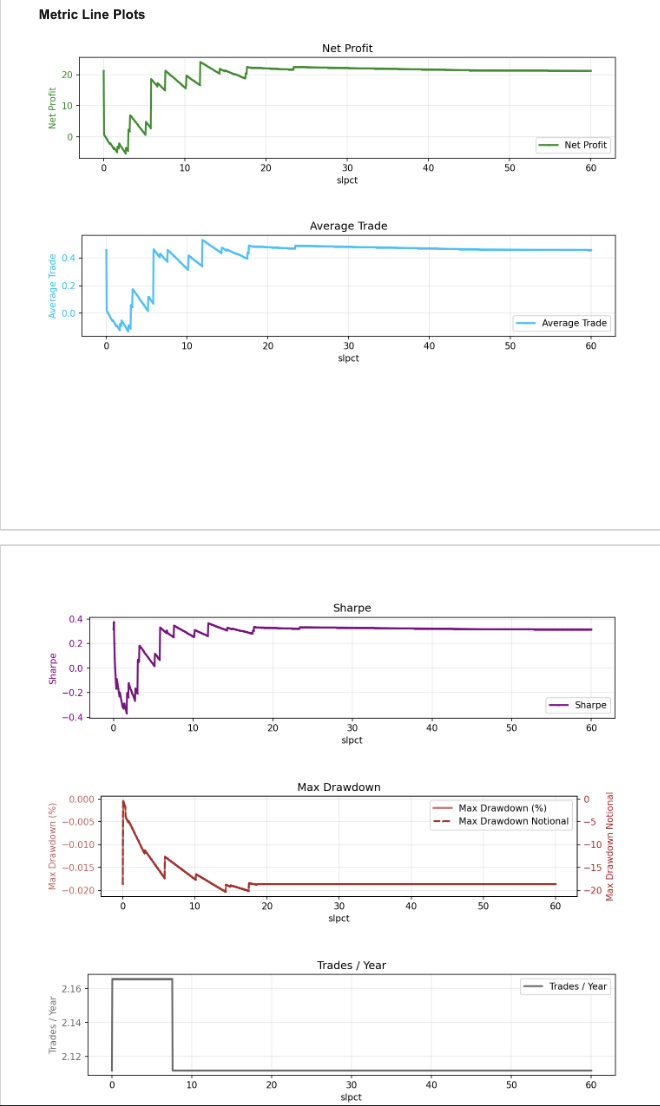
\includegraphics[height=0.44\textheight]{figures/opt/macross/slpct.png} &
        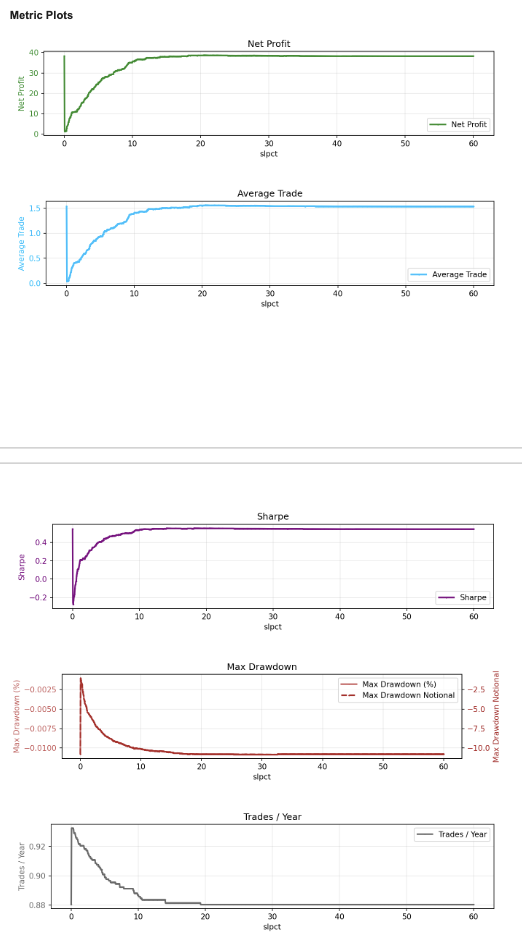
\includegraphics[height=0.44\textheight]{figures/opt/macross/syn_slpct.png}
    \end{tabular}

    \caption{Moving-average crossover: stop-loss optimization. Left: historical IS. Right: synthetic mean.}
    \label{fig:mac-slpct}
    \label{fig:mac-slpct-syn}
\end{figure}

The synthetic plot has a similar shape to the historical one, but it is smoother. This is expected,
since every point is averaged across 50 paths instead of being measured on one path only.

The stop-loss was left disabled (\(slpct = -1\)) for both the benchmark and the synthetic configuration
because short stop-loss values produced unstable results.

\subsection{Fast/slow length stage}

With the stop-loss disabled, the fast and slow moving-average lengths were optimized jointly.
Figures~\ref{fig:mac-mas}--\ref{fig:mac-ms2} compare the historical-IS grid with the synthetic-path
mean.

\begin{figure}[H]
    \centering

    \begin{minipage}{0.49\textwidth}
        \centering
        \textbf{Historical IS}\\[0.2em]
        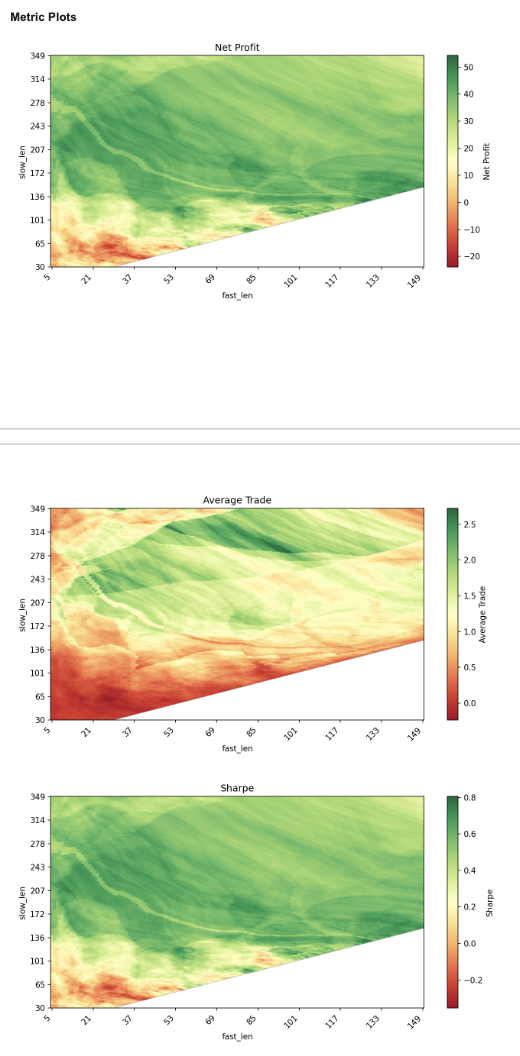
\includegraphics[width=\linewidth]{figures/opt/macross/mas.png}
    \end{minipage}
    \hfill
    \begin{minipage}{0.49\textwidth}
        \centering
        \textbf{Synthetic mean}\\[0.2em]
        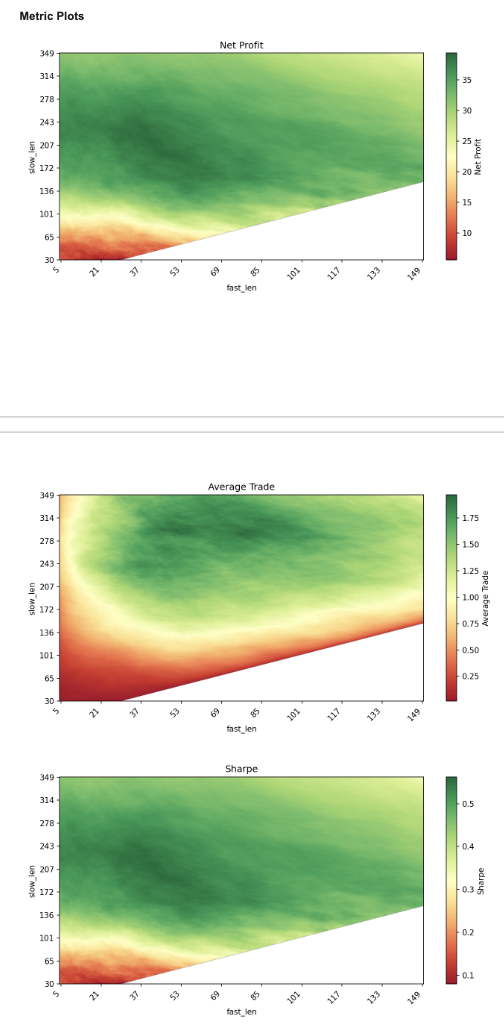
\includegraphics[width=\linewidth]{figures/opt/macross/syn_mas.png}
    \end{minipage}

    \caption{Moving-average crossover: first metric panel over the fast/slow length grid.}
    \label{fig:mac-mas}
    \label{fig:mac-syn-mas}
\end{figure}

\begin{figure}[H]
    \centering

    \begin{minipage}{0.49\textwidth}
        \centering
        \textbf{Historical IS}\\[0.2em]
        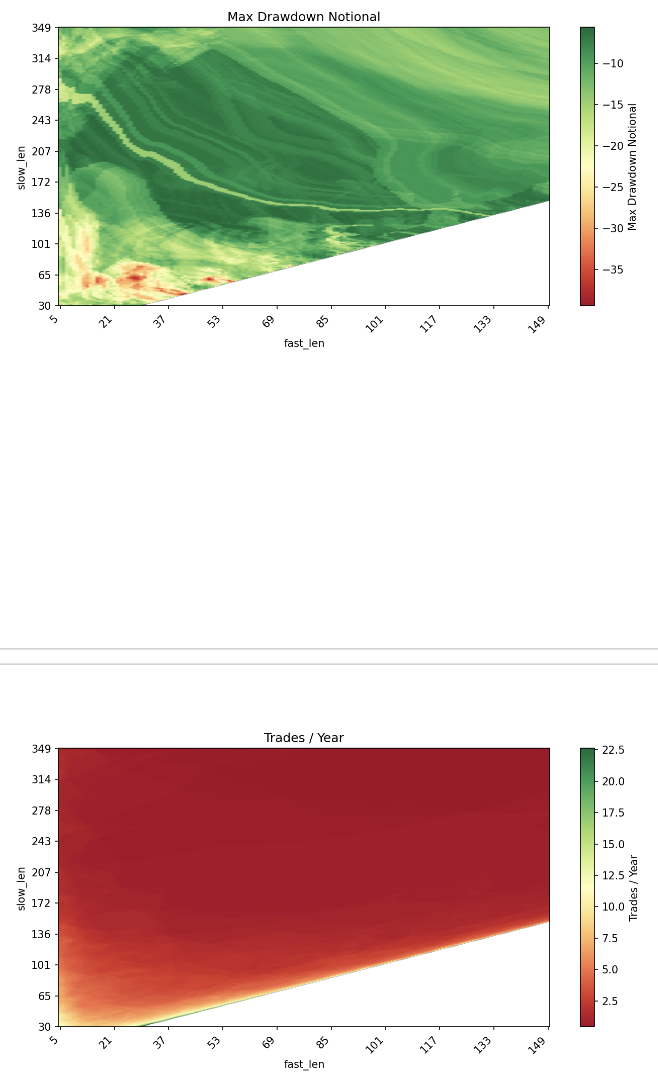
\includegraphics[width=\linewidth]{figures/opt/macross/ms2.png}
    \end{minipage}
    \hfill
    \begin{minipage}{0.49\textwidth}
        \centering
        \textbf{Synthetic mean}\\[0.2em]
        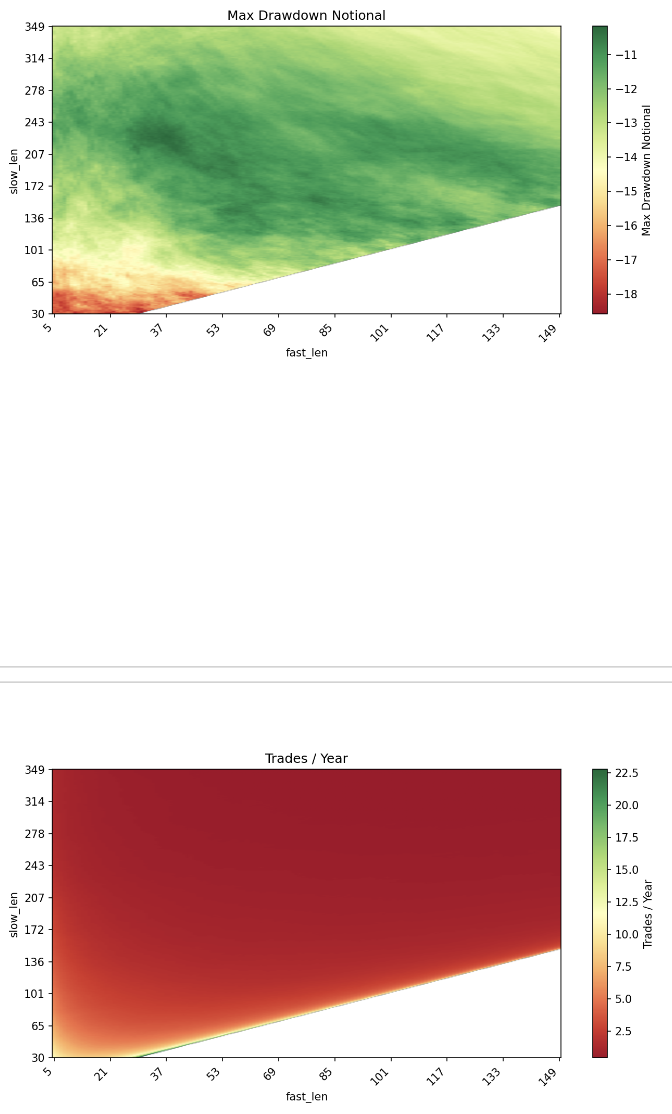
\includegraphics[width=\linewidth]{figures/opt/macross/syn_mas2.png}
    \end{minipage}

    \caption{Moving-average crossover: second metric panel over the fast/slow length grid.}
    \label{fig:mac-ms2}
    \label{fig:mac-syn-ms2}
\end{figure}

Both grids show the same main pattern. Results are weak when the fast and slow lengths are close,
because the strategy trades too often on small price moves. Results improve when the slow length is
larger, creating a broad stable area near \(slow\_len = 200\). From this region, I chose
\(fast\_len = 50\), \(slow\_len = 200\) for the benchmark configuration. For the synthetic
configuration, I kept the same slow length but chose a shorter fast length:
\(fast\_len = 35\), \(slow\_len = 200\).

\section{Standard-deviation mean-reversion optimization}

\subsection{Stop-loss stage}

As with the crossover strategy, the stop-loss percentage was optimized first, holding the
standard-deviation length and thresholds at their resting values (\(std\_len = 15\),
\(lower\_std\_thresh = -1.5\), \(upper\_std\_thresh = 1.5\)). Figure~\ref{fig:mrev-slpct} sweeps the
stop-loss percentage from 0\% to 60\% on the real historical IS period.

\begin{figure}[H]
    \centering
    
\includegraphics[width=0.85\textwidth]{figures/opt/mrev/slpct.png}
    \caption{Std MRev: metrics as a function of the stop-loss percentage, historical IS.}
    \label{fig:mrev-slpct}
\end{figure}

For this strategy, the stop-loss curve has a clearer structure. Net profit and Sharpe improve for small
stop-loss values, around 1\%--3\%, then deteriorate and eventually flatten once the stop is so wide that
it rarely triggers. That flat region is stable, but it is not useful: a mean-reversion trade should be
cut when the move keeps going against it. For this reason, the benchmark stop-loss was selected from the
early profitable region, giving \(slpct = 2.5\%\). This is a risk-control choice, not a pure
maximum-metric choice.

The same sweep was repeated on synthetic paths, holding the same resting values.
Figures~\ref{fig:mrev-syn-slpct-np}--\ref{fig:mrev-syn-slpct-sharpe} report the synthetic-path mean.

\begin{figure}[H]
    \centering

    \begin{minipage}{0.49\textwidth}
        \centering
        \textbf{Net profit}\\[0.2em]
        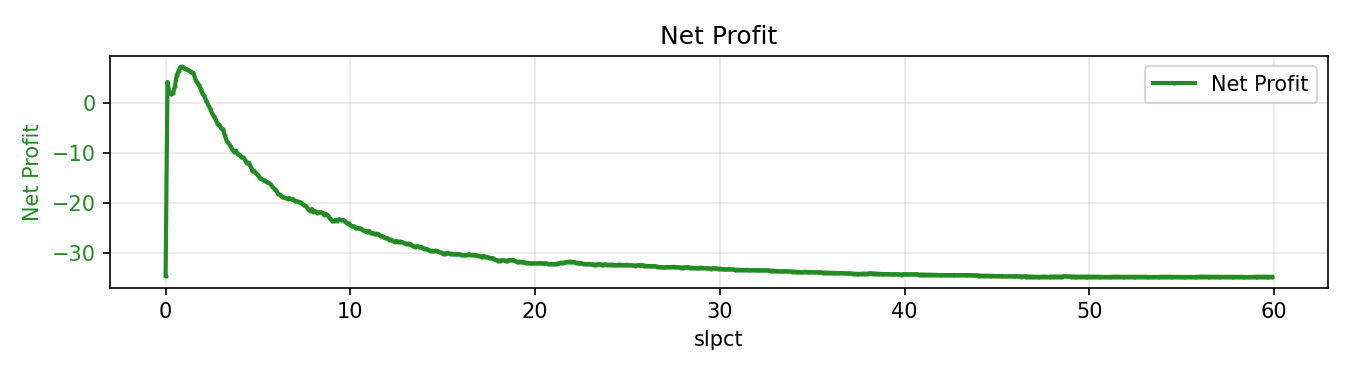
\includegraphics[width=\linewidth]{figures/opt/mrev/syn_slpct_net_profit.png}
    \end{minipage}
    \hfill
    \begin{minipage}{0.49\textwidth}
        \centering
        \textbf{Sharpe}\\[0.2em]
        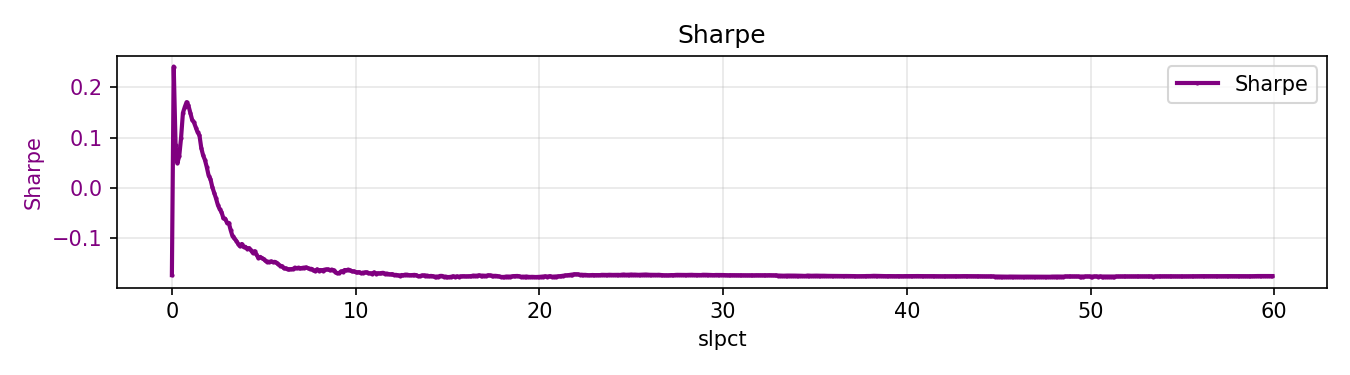
\includegraphics[width=\linewidth]{figures/opt/mrev/syn_slpct_sharpe.png}
    \end{minipage}

    \caption{Std MRev: stop-loss optimization, mean over synthetic paths.}
    \label{fig:mrev-syn-slpct-np}
    \label{fig:mrev-syn-slpct-sharpe}
\end{figure}

Averaging over synthetic paths removes most of the noise. The curve rises near the 1\% area and then
decays toward the same inactive-stop plateau. The best single point, \(slpct = 0.1\%\), is too isolated
to use directly. Using the same risk-control logic as above, the synthetic configuration uses
\(slpct = 2.0\%\).

\subsection{Length and linked threshold stage}

With the stop-loss fixed, I optimized the standard-deviation length together with one threshold level.
To avoid optimizing the length alone, but also avoid a three-parameter grid, the upper and lower
thresholds were linked symmetrically: one positive threshold for short entries and one negative
threshold of the same size for long entries.
Figure~\ref{fig:mrev-sllen1} compares the main historical-IS grid with the synthetic-path mean.
Figure~\ref{fig:mrev-sllen2} shows the trades/year surface for the historical-IS grid, since it helps
explain how the optimization process was interpreted. The synthetic version was very similar, so it is
not repeated here.

\begin{figure}[H]
    \centering

    \begin{minipage}{0.49\textwidth}
        \centering
        \textbf{Historical IS}\\[0.2em]
        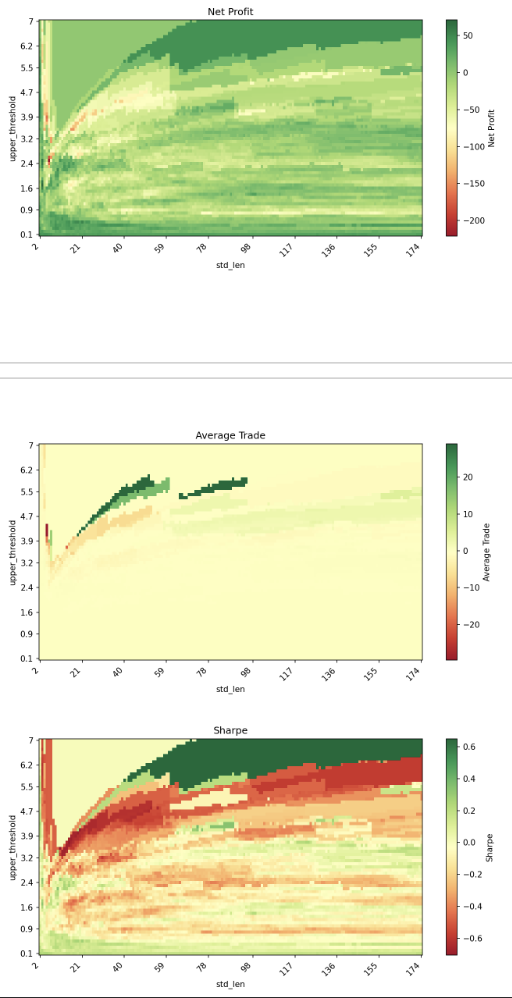
\includegraphics[width=\linewidth]{figures/opt/mrev/sllen_thresh.png}
    \end{minipage}
    \hfill
    \begin{minipage}{0.49\textwidth}
        \centering
        \textbf{Synthetic mean}\\[0.2em]
        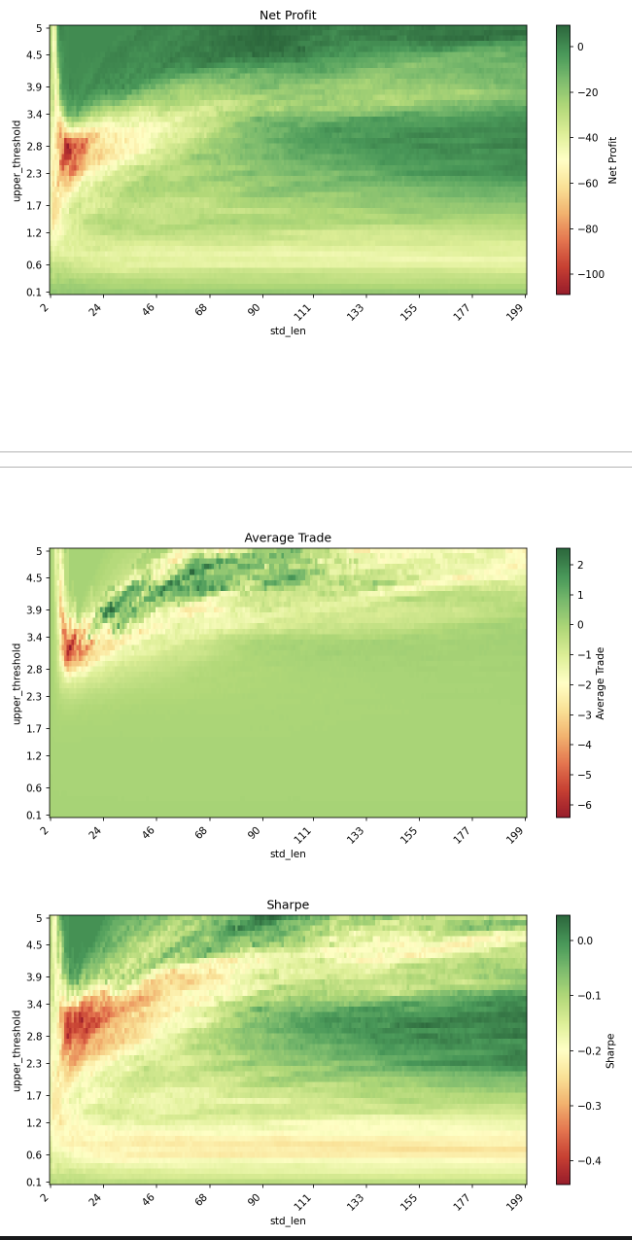
\includegraphics[width=\linewidth]{figures/opt/mrev/syn_slen_thresh.png}
    \end{minipage}

    \caption{Std MRev: first metric panel over the length/symmetric-threshold grid.}
    \label{fig:mrev-sllen1}
    \label{fig:mrev-syn-sllen}
\end{figure}

\begin{figure}[H]
    \centering
    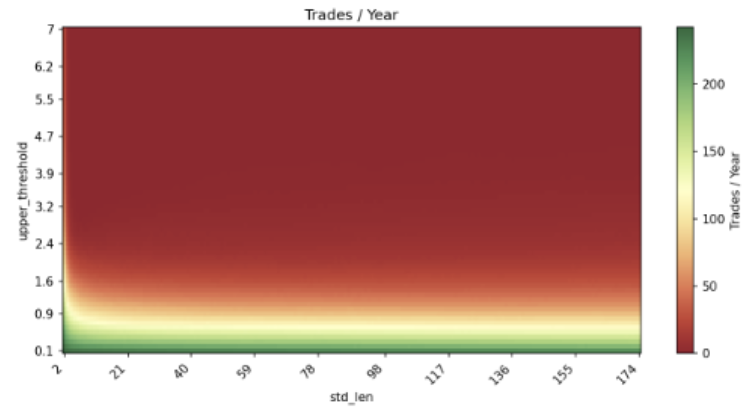
\includegraphics[width=0.85\textwidth]{figures/opt/mrev/show_in_5.7_instead_of_second_img.png}
    \caption{Std MRev: trades per year over the length/symmetric-threshold grid, historical IS.}
    \label{fig:mrev-sllen2}
\end{figure}

Very short standard-deviation lengths perform poorly because they react to almost every local move. In
the historical grid, performance becomes usable around 20--40 bars, so the benchmark configuration uses
\(std\_len = 20\) and a narrow symmetric threshold as the starting point. In the synthetic grid, the
stable area appears much later, around 100--150 bars, with a wider threshold. The synthetic
configuration therefore uses \(std\_len = 150\) and starts from a wider threshold. The symmetric
threshold is only an intermediate step; the final stage separates the upper and lower thresholds.

\subsection{Independent threshold stage}

Finally, the upper and lower thresholds were optimized independently, holding the standard-deviation
length and stop-loss at the values selected in the previous stages. Figure~\ref{fig:mrev-tt} compares
the main historical-IS grid at \(std\_len = 20\) with the synthetic-path mean at \(std\_len = 150\).
Figure~\ref{fig:mrev-syn-tt2} shows the trades/year surface to make the optimization process easier to
read. The benchmark and synthetic trades/year plots were very similar, so only this one is reported.

\begin{figure}[H]
    \centering

    \begin{minipage}{0.49\textwidth}
        \centering
        \textbf{Historical IS}\\[0.2em]
        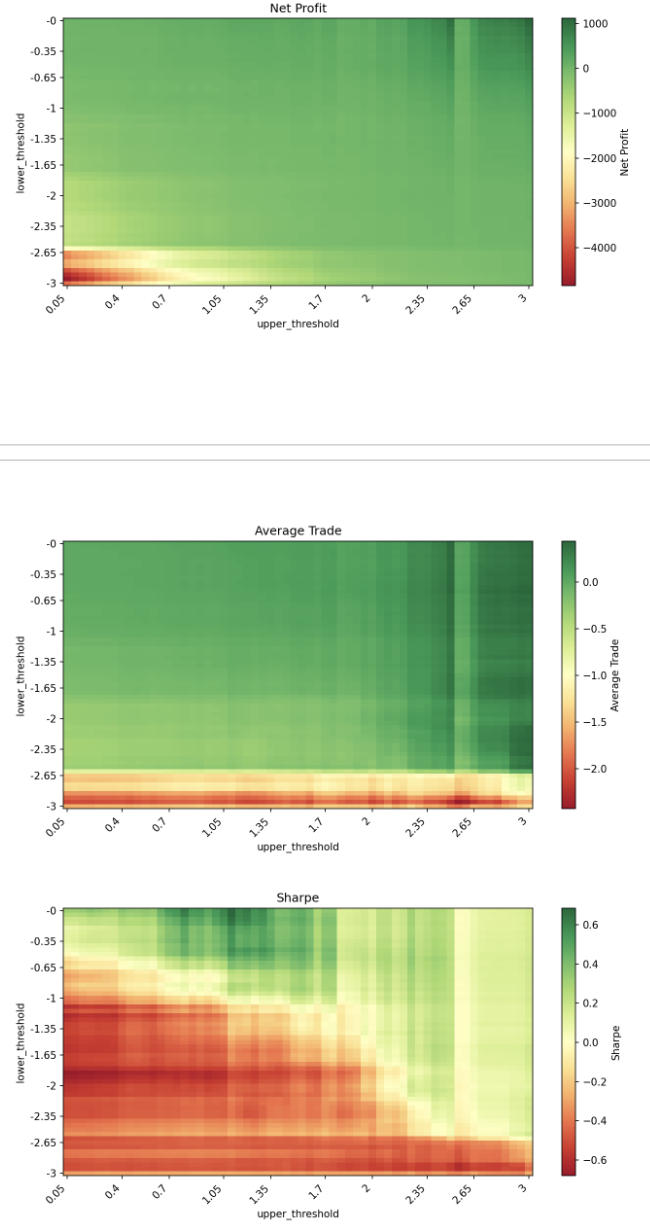
\includegraphics[width=\linewidth]{figures/opt/mrev/thresh_thresh.png}
    \end{minipage}
    \hfill
    \begin{minipage}{0.49\textwidth}
        \centering
        \textbf{Synthetic mean}\\[0.2em]
        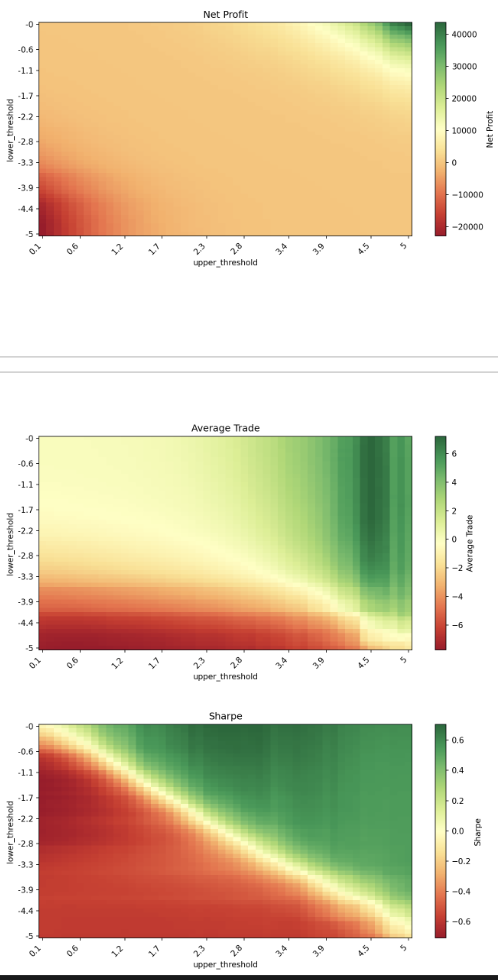
\includegraphics[width=\linewidth]{figures/opt/mrev/syn_thresh_thresh.png}
    \end{minipage}

    \caption{Std MRev: first metric panel over the independent upper/lower threshold grid.}
    \label{fig:mrev-tt}
    \label{fig:mrev-syn-tt1}
\end{figure}

Figure~\ref{fig:mrev-tt} is one of the clearest examples of why the synthetic-path mean is useful. In
particular, the Sharpe surface is much smoother on the synthetic side. Averaging across paths appears to
cancel part of the single-path noise and makes the stable region easier to see, although the two panels
come from the parameter settings used in each workflow.

\begin{figure}[H]
    \centering
    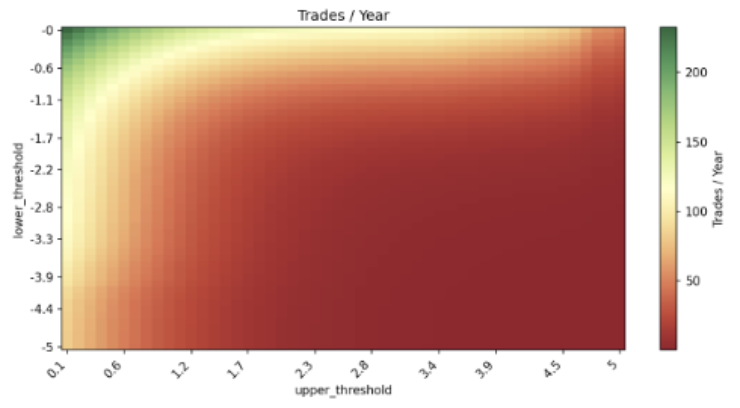
\includegraphics[width=0.85\textwidth]{figures/opt/mrev/show_in_5.9.png}
    \caption{Std MRev: trades per year over the independent upper/lower threshold grid.}
    \label{fig:mrev-syn-tt2}
\end{figure}

The independent-threshold grids show that the symmetric rule is not ideal. Performance improves when
the lower threshold is kept close to zero and the upper threshold is wider. The final benchmark
thresholds are \(upper\_std\_thresh = 1.0\), \(lower\_std\_thresh = -0.35\). The final synthetic
thresholds are \(upper\_std\_thresh = 3.0\), \(lower\_std\_thresh = -0.30\). In both cases, the strategy
becomes more sensitive to downside moves than upside moves.

\section{Selected parameters}

Table~\ref{tab:selected-params} summarizes the selected parameters. These configurations are fixed and
then evaluated on the real OOS period in the following chapter.

\begin{table}[H]
    \centering
    \begin{tabular}{lllll}
        \toprule
        Strategy & Method & Parameters & slpct & Other \\
        \midrule
        MA Cross & Benchmark & fast=50, slow=200 & disabled & -- \\
        MA Cross & Synthetic & fast=35, slow=200 & disabled & -- \\
        Std MRev & Benchmark & std\_len=20 & 2.5\% & upper=1.0, lower=-0.35 \\
        Std MRev & Synthetic & std\_len=150 & 2.0\% & upper=3.0, lower=-0.30 \\
        \bottomrule
    \end{tabular}
    \caption{Final selected parameters per strategy and optimization method.}
    \label{tab:selected-params}
\end{table}

Both methods use the same optimization process: parameters are chosen from robust grid regions rather
than isolated peaks. The difference is the optimization data: the benchmark uses the real historical IS
period, while the synthetic method uses the mean result across synthetic IS paths. The real test is the
next step: comparing IS-to-OOS deterioration and checking whether the synthetic method reduces it.


\chapter{Results}
This chapter reports and discusses the empirical results obtained from historical backtests, optimization experiments, and synthetic market comparisons.



\chapter{Conclusion}
This chapter summarizes the main findings, limitations, and possible future improvements.


\chapter*{Code Availability}
\addcontentsline{toc}{chapter}{Code Availability}

All code used for this thesis was developed independently by the author and is publicly available at:
\url{https://github.com/JacopoMichelacci/100_OOS_BSc_Thesis}.

The thesis focuses on the research design, optimization procedure, synthetic market generation, and
empirical results. For this reason, implementation details are discussed only when they are necessary
to understand the methodology. The full source code is provided in the repository for reproducibility
and further inspection.

\begin{thebibliography}{9}
\addcontentsline{toc}{chapter}{References}

\bibitem{politis1994}
Politis, D. N., and Romano, J. P. (1994).
The stationary bootstrap.
\textit{Journal of the American Statistical Association}, 89(428), 1303--1313.

\bibitem{white2000}
White, H. (2000).
A reality check for data snooping.
\textit{Econometrica}, 68(5), 1097--1126.

\bibitem{bailey2017}
Bailey, D. H., Borwein, J. M., L\'opez de Prado, M., and Zhu, Q. J. (2017).
The probability of backtest overfitting.
\textit{Journal of Computational Finance}, 20(4), 39--69.

\end{thebibliography}

\end{document}
